\section{Language}\label{sec:language}
This section describes the domain specific language built upon the language model described in Section~\ref{sec:model}. First the deployment of the language is provided that explains how the DSL is operates and is used in usage management systems. This is followed by a detailed example of the syntax and semantics, and major components of the language. Finally, we demonstrate how the language can be extended to include different types of evaluators deploying different types of logics. 

\begin{figure}[!t]
\centering
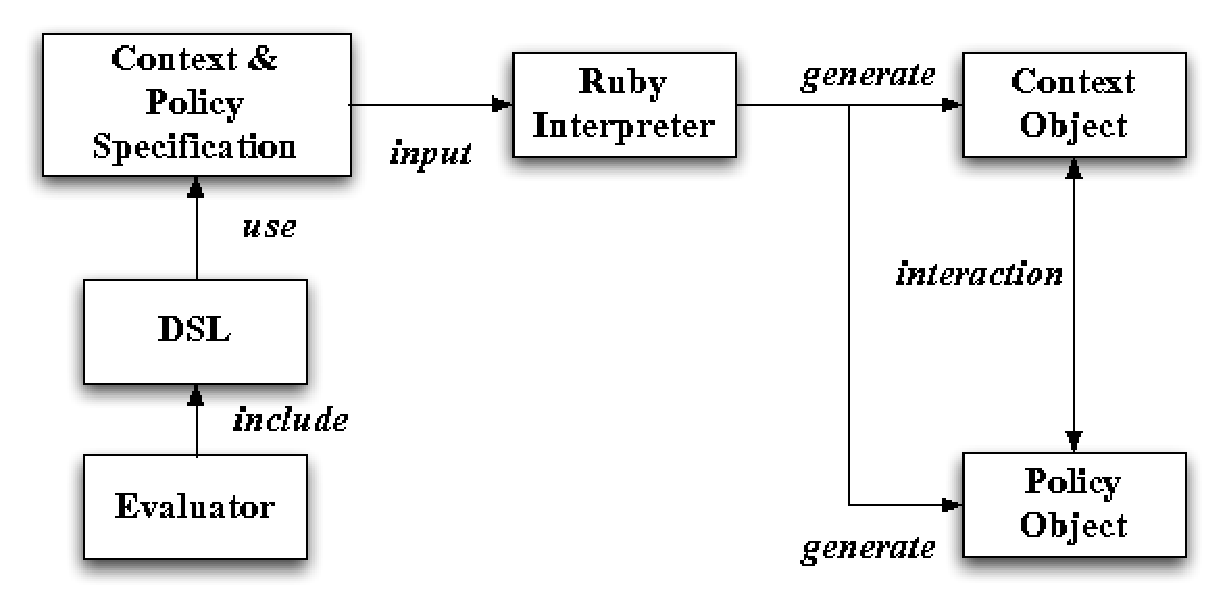
\includegraphics[width=3.5in]{DSL-usage}
\caption{The role of DSL in usage management systems}
\label{fig:DSL-usage}
\end{figure}

\subsection{Language Operation}
The use and operation of the DSL for usage management is shown in Figure~\ref{fig:DSL-usage}. The DSL provides a language for specification of contexts and policies as described in the previous section. As shown in the figure, the DSL can incorporate different types of evaluators for expression of different types of usage semantics. A DSL, along with an appropriate evaluator is then used to specify contexts and policies. Users are allowed to choose from different types of evaluators that provide the right type of semantics needed by the users. The policy specification and context specification, described using the DSL is then taken by a Ruby compiler to generate a corresponding context and policy object. In usage management systems, context objects are generated on the client side and maintained within the computing platform. The policy specification is provided by the resource owners, is converted into a policy object. Following this, the policy and context objects interact with each other and operate within a usage management system.  

\subsection{Language Description}
The language is based on the model description provided in the previous section, and enables specification of the various policy semantics and context descriptions. 

\subsubsection{Context Specification}

The DSL provides a mechanism for specification of different types of contexts based on the context structure explained in the previous section. A context consists of a set of entities, such as Subject, Resource, and Environment, and each of these entities possess a set of properties. Every property supports a set of functions that operate over the property. The steps involved in defining a context first includes the description of different types of properties. The properties are then allocated to different entities, and then entities are assigned to a given context. 

\begin{table*}[t]
\caption{An example structure of context.}
\label{table:context}
\begin{center}
{\scriptsize
\begin{tabular}{|c|c|c|c|}
\hline
\multicolumn{4}{|c|}{ \bf Context}\\
\hline
{ \bf Entity} & {\bf Property ($p$)} & { \bf Domain ($D_p$)} & {\bf Functions ($F_p$)}\\
\hline
\multirow{3}{*}{Environment (E)} & OperatingSystem & \{Windows, OSX, SELinux\}&  equatable\\
                                                    & Device & \{Workstation, Handheld, Blackberry, Terminal\} & equatable \\
                                                    & SecurityDomain & \{ ABNet, SECNet, TELNet, OMNINet\} & comparable\\ 
\hline
\multirow{3}{*}{Subject (S)} & SecurityClearance & \{Top Secret, Secret, Confidential\} &  comparable\\
				      &Project & \{Zebra, Yuma, Lion\} & equatable\\
				       &Role & \{Alpha, Beta, Delta\} & equatable\\

\hline
 Resource(R) & SecurityClassification & \{ Top Secret, Secret, Confidential, Unclassified\} & comparable \\
\hline

\end{tabular}
}
\end{center}
\label{default}
\end{table*} 

Consider a multi-level security context as shown in Table~\ref{table:context}. The context consists of two entities, namely, {\em Subject} and {\em Environment} and {\em Resource}. {\em Subject} entity has three properties, namely, {\em Security Clearance}, {\em Role} and {\em Project}. {\em Environment} entity has three properties, namely, {\em OperatingSystem}, {\em Device} and {\em SecurityDomain}. {\em Resource} entity has one property,{SecurityClassification}. Every property supports a set of functions depending on the type of that property. For the purpose of this discussion, we explain two types of properties, namely, equatable and comparable. Equatable properties primarily support equality functions  ``$=$" and ``$!=$". Comparable properties support functions that allow relative comparison of two values, namely, ``$=$" , ``$!=$", ``$<$", ``$>$",  ``$\leq$", ``$\geq$" and ``$between()$". Both, equatable and comparable property types support ``$get()$" and ``$set()$" functions to retrieve and set property values. The properties {\em OperatingSystem}, {\em Device}, {\em Project} and {\em Role} are equatable properties, and {\em SecurityDomain}, {\em SecurityClearance} and {\em SecurityClassfication} are comparable properties. {\em SecurityDomain} property values have the ordering $ABNet > SECNet > TELNet > OMNINet$,  {\em SecurityClearance} property values have the ordering $Top\;Secret > Secret > Confidential$, and {\em SecurityClassification} property values have the ordering $Top\;Secret > Secret > Confidential > Unclassified$. 

In order to specify this context, individual properties are defined first as follows. 

\begin{tabbing}
             property \= (:OperatingSystem) {\bf do} \\
\>	   {\bf values}  :Windows, :OSX,  :SELinux\\
\>	   {\bf functions}   :set, :get, :equatable \\
	{\bf end} 
\end{tabbing}
	
\begin{tabbing}
 property \= (:Device) {\bf do} \\
\>	 {\bf values} \= :Workstation, :Handheld, :Blackberry, \\
\>\>      :Terminal\\
\>	 {\bf functions}  :set, :get, :equatable \\
	 {\bf end}
\end{tabbing}

\begin{tabbing}
property \= (:Project) {\bf do} \\
\>	 {\bf values}  :Zebra, :Yuma, :Lion\\
\>	 {\bf functions} :set, :get, :equatable \\
	 {\bf end}
\end{tabbing}

\begin{tabbing}	
 property  \= (:Role) {\bf do} \\
\>	 {\bf values} :Alpha, :Beta, :Delta\\
\>	 {\bf functions}  :set, :get, :equatable \\
	 {\bf end}
\end{tabbing}
	
In this example, classes  {\em OperatingSystem, Device, Project} and {\em Role} that inherit the type {\em property} are specified. The term {\em values} specify the set of valid values and {\em functions} define the set of functions supported by the class as described earlier. Similarly, classes for comparable properties are defined, with the addition that the ordering of the valid values is specified by the user as shown below. 

\begin{tabbing}
             property \= (:SecurityDomain) {\bf do} \\
\>	   {\bf values}  :ABNet, :SECNet, :TELNet, :OMNINet\\
\>	   {\bf functions}   :set, :get, :comparable \\
\>	   {\bf order} :ABNet > :SecNet > :TELNet > :OMNINet\\
	{\bf end} 
\end{tabbing}
	
\begin{tabbing}
 property \= (:SecurityClearance) {\bf do} \\
\>	 {\bf values} \= :Top Secret, :Secret, :Confidential \\
\>	 {\bf functions}  :set, :get, :comparable \\
\>       {\bf order} :Top Secret > Secret > Confidential
	 {\bf end}
\end{tabbing}

\begin{tabbing}
property \= (:SecurityClassification) {\bf do} \\
\>	 {\bf values} \=  :Top Secret, :Secret, :Confidential, \\
\>\>                               :Unclassified\\
\>	 {\bf functions} :set, :get, :comparable \\
\>       {\bf order} \= :Top Secret > :Secret > Confidential > \\
\>\>                           Unclassified\\
	 {\bf end}
\end{tabbing}







\subsection{Langauge Extensions}

The DSL allows inclusion of different types of evaluators that provide users with different sets of usage semantics. The evaluators provide a design space for innovation and extensibility



